% Options for packages loaded elsewhere
\PassOptionsToPackage{unicode}{hyperref}
\PassOptionsToPackage{hyphens}{url}
%
\documentclass[
  12pt,
  landscape]{article}
\usepackage{lmodern}
\usepackage{amssymb,amsmath}
\usepackage{ifxetex,ifluatex}
\ifnum 0\ifxetex 1\fi\ifluatex 1\fi=0 % if pdftex
  \usepackage[T1]{fontenc}
  \usepackage[utf8]{inputenc}
  \usepackage{textcomp} % provide euro and other symbols
\else % if luatex or xetex
  \usepackage{unicode-math}
  \defaultfontfeatures{Scale=MatchLowercase}
  \defaultfontfeatures[\rmfamily]{Ligatures=TeX,Scale=1}
\fi
% Use upquote if available, for straight quotes in verbatim environments
\IfFileExists{upquote.sty}{\usepackage{upquote}}{}
\IfFileExists{microtype.sty}{% use microtype if available
  \usepackage[]{microtype}
  \UseMicrotypeSet[protrusion]{basicmath} % disable protrusion for tt fonts
}{}
\makeatletter
\@ifundefined{KOMAClassName}{% if non-KOMA class
  \IfFileExists{parskip.sty}{%
    \usepackage{parskip}
  }{% else
    \setlength{\parindent}{0pt}
    \setlength{\parskip}{6pt plus 2pt minus 1pt}}
}{% if KOMA class
  \KOMAoptions{parskip=half}}
\makeatother
\usepackage{xcolor}
\IfFileExists{xurl.sty}{\usepackage{xurl}}{} % add URL line breaks if available
\IfFileExists{bookmark.sty}{\usepackage{bookmark}}{\usepackage{hyperref}}
\hypersetup{
  pdftitle={ECON 21110 - Applied Microeconometrics - Assignment 3},
  pdfauthor={Jack Ogle in collaboration with Eva Haque, Matt Lohrs, and Jack Knickrehm},
  hidelinks,
  pdfcreator={LaTeX via pandoc}}
\urlstyle{same} % disable monospaced font for URLs
\usepackage[margin=1in]{geometry}
\usepackage{color}
\usepackage{fancyvrb}
\newcommand{\VerbBar}{|}
\newcommand{\VERB}{\Verb[commandchars=\\\{\}]}
\DefineVerbatimEnvironment{Highlighting}{Verbatim}{commandchars=\\\{\}}
% Add ',fontsize=\small' for more characters per line
\usepackage{framed}
\definecolor{shadecolor}{RGB}{248,248,248}
\newenvironment{Shaded}{\begin{snugshade}}{\end{snugshade}}
\newcommand{\AlertTok}[1]{\textcolor[rgb]{0.94,0.16,0.16}{#1}}
\newcommand{\AnnotationTok}[1]{\textcolor[rgb]{0.56,0.35,0.01}{\textbf{\textit{#1}}}}
\newcommand{\AttributeTok}[1]{\textcolor[rgb]{0.77,0.63,0.00}{#1}}
\newcommand{\BaseNTok}[1]{\textcolor[rgb]{0.00,0.00,0.81}{#1}}
\newcommand{\BuiltInTok}[1]{#1}
\newcommand{\CharTok}[1]{\textcolor[rgb]{0.31,0.60,0.02}{#1}}
\newcommand{\CommentTok}[1]{\textcolor[rgb]{0.56,0.35,0.01}{\textit{#1}}}
\newcommand{\CommentVarTok}[1]{\textcolor[rgb]{0.56,0.35,0.01}{\textbf{\textit{#1}}}}
\newcommand{\ConstantTok}[1]{\textcolor[rgb]{0.00,0.00,0.00}{#1}}
\newcommand{\ControlFlowTok}[1]{\textcolor[rgb]{0.13,0.29,0.53}{\textbf{#1}}}
\newcommand{\DataTypeTok}[1]{\textcolor[rgb]{0.13,0.29,0.53}{#1}}
\newcommand{\DecValTok}[1]{\textcolor[rgb]{0.00,0.00,0.81}{#1}}
\newcommand{\DocumentationTok}[1]{\textcolor[rgb]{0.56,0.35,0.01}{\textbf{\textit{#1}}}}
\newcommand{\ErrorTok}[1]{\textcolor[rgb]{0.64,0.00,0.00}{\textbf{#1}}}
\newcommand{\ExtensionTok}[1]{#1}
\newcommand{\FloatTok}[1]{\textcolor[rgb]{0.00,0.00,0.81}{#1}}
\newcommand{\FunctionTok}[1]{\textcolor[rgb]{0.00,0.00,0.00}{#1}}
\newcommand{\ImportTok}[1]{#1}
\newcommand{\InformationTok}[1]{\textcolor[rgb]{0.56,0.35,0.01}{\textbf{\textit{#1}}}}
\newcommand{\KeywordTok}[1]{\textcolor[rgb]{0.13,0.29,0.53}{\textbf{#1}}}
\newcommand{\NormalTok}[1]{#1}
\newcommand{\OperatorTok}[1]{\textcolor[rgb]{0.81,0.36,0.00}{\textbf{#1}}}
\newcommand{\OtherTok}[1]{\textcolor[rgb]{0.56,0.35,0.01}{#1}}
\newcommand{\PreprocessorTok}[1]{\textcolor[rgb]{0.56,0.35,0.01}{\textit{#1}}}
\newcommand{\RegionMarkerTok}[1]{#1}
\newcommand{\SpecialCharTok}[1]{\textcolor[rgb]{0.00,0.00,0.00}{#1}}
\newcommand{\SpecialStringTok}[1]{\textcolor[rgb]{0.31,0.60,0.02}{#1}}
\newcommand{\StringTok}[1]{\textcolor[rgb]{0.31,0.60,0.02}{#1}}
\newcommand{\VariableTok}[1]{\textcolor[rgb]{0.00,0.00,0.00}{#1}}
\newcommand{\VerbatimStringTok}[1]{\textcolor[rgb]{0.31,0.60,0.02}{#1}}
\newcommand{\WarningTok}[1]{\textcolor[rgb]{0.56,0.35,0.01}{\textbf{\textit{#1}}}}
\usepackage{graphicx,grffile}
\makeatletter
\def\maxwidth{\ifdim\Gin@nat@width>\linewidth\linewidth\else\Gin@nat@width\fi}
\def\maxheight{\ifdim\Gin@nat@height>\textheight\textheight\else\Gin@nat@height\fi}
\makeatother
% Scale images if necessary, so that they will not overflow the page
% margins by default, and it is still possible to overwrite the defaults
% using explicit options in \includegraphics[width, height, ...]{}
\setkeys{Gin}{width=\maxwidth,height=\maxheight,keepaspectratio}
% Set default figure placement to htbp
\makeatletter
\def\fps@figure{htbp}
\makeatother
\setlength{\emergencystretch}{3em} % prevent overfull lines
\providecommand{\tightlist}{%
  \setlength{\itemsep}{0pt}\setlength{\parskip}{0pt}}
\setcounter{secnumdepth}{-\maxdimen} % remove section numbering
\usepackage{dcolumn}
\usepackage{float}

\title{ECON 21110 - Applied Microeconometrics - Assignment 3}
\author{Jack Ogle in collaboration with Eva Haque, Matt Lohrs, and Jack
Knickrehm}
\date{}

\begin{document}
\maketitle

Problem 1

\begin{enumerate}
\def\labelenumi{(\alph{enumi})}
\item
\end{enumerate}

Banerjee, Cole, Duflo, and Liden are trying to understand two opposing
ideas about education. (1) According to the Millennium Development Goals
put forth by the United Nations, primary education should be a universal
right. (2) However, the quality of education currently offered to the
poor is of bad quality. These authors are trying to understand why the
children of poor countries are receiving inferior education. They
conduct a field experiment where they measure the effect of the Balsakhi
Program and CAL the (Computer Assisted Learning) Program on the learning
levels of elementary school children in India. The students learning
levels are measured by mathematical and verbal standardized tests. The
students take the tests pre and post treatment.

\begin{enumerate}
\def\labelenumi{(\alph{enumi})}
\setcounter{enumi}{1}
\item
\end{enumerate}

To ensure a balanced sample, assignment was stratified by language,
pretest score, and gender.

We stratify the pretest scores and gender like they did in the study. We
can accomplish this by regressing the balsakhi on the male and bal
variable. Which gives us the following result. We see that the pre\_tot
coefficient is -0.0002 close to zero, and are statistically significant.
We can also see that the male coefficient is close to 0 and not
statistically significant. We can conclude that the treatment and
control groups are balanced because the effect of gender and pretest
scores have very little effect on whether a student is placed in the
treatment or control group. Yes, we should cluster standard errors and
they are labeled in the table.

\begin{table}[H] \centering 
  \caption{Regression Results (b)} 
  \label{} 
\begin{tabular}{@{\extracolsep{5pt}}lD{.}{.}{-3} D{.}{.}{-3} } 
\\[-1.8ex]\hline 
\hline \\[-1.8ex] 
 & \multicolumn{2}{c}{\textit{Dependent variable:}} \\ 
\cline{2-3} 
\\[-1.8ex] & \multicolumn{2}{c}{bal} \\ 
 & \multicolumn{1}{c}{Without Clustered Std. Errors} & \multicolumn{1}{c}{With Clustered Std. Errors} \\ 
\\[-1.8ex] & \multicolumn{1}{c}{(1)} & \multicolumn{1}{c}{(2)}\\ 
\hline \\[-1.8ex] 
 pre\_tot & -0.0002 & -0.0002 \\ 
  & (0.0002) & (0.0009) \\ 
  & & \\ 
 male & 0.018^{*} & 0.018^{*} \\ 
  & (0.010) & (0.0431) \\ 
  & & \\ 
 Constant & 0.485^{***} & 0.485^{***} \\ 
  & (0.010) & (0.0524) \\ 
  & & \\ 
\hline \\[-1.8ex] 
Observations & \multicolumn{1}{c}{9,745} & \multicolumn{1}{c}{9,745} \\ 
R$^{2}$ & \multicolumn{1}{c}{0.0004} & \multicolumn{1}{c}{0.0004} \\ 
Adjusted R$^{2}$ & \multicolumn{1}{c}{0.0002} & \multicolumn{1}{c}{0.0002} \\ 
Residual Std. Error (df = 9742) & \multicolumn{1}{c}{0.500} & \multicolumn{1}{c}{0.500} \\ 
F Statistic (df = 2; 9742) & \multicolumn{1}{c}{1.934} & \multicolumn{1}{c}{1.934} \\ 
\hline 
\hline \\[-1.8ex] 
\textit{Note:}  & \multicolumn{2}{l}{$^{*}$p$<$0.1; $^{**}$p$<$0.05; $^{***}$p$<$0.01} \\ 
 & \multicolumn{2}{l}{Standard errors in parentheses} \\ 
\end{tabular} 
\end{table}

\begin{enumerate}
\def\labelenumi{(\alph{enumi})}
\setcounter{enumi}{2}
\item
\end{enumerate}

\begin{table}[H] \centering 
  \caption{Regression Results (c)} 
  \label{} 
\begin{tabular}{@{\extracolsep{5pt}}lD{.}{.}{-3} D{.}{.}{-3} D{.}{.}{-3} D{.}{.}{-3} } 
\\[-1.8ex]\hline 
\hline \\[-1.8ex] 
 & \multicolumn{4}{c}{\textit{Dependent variable:}} \\ 
\cline{2-5} 
\\[-1.8ex] & \multicolumn{4}{c}{bal} \\ 
 & \multicolumn{1}{c}{Pretest Treatment} & \multicolumn{1}{c}{Pretest Comparision} & \multicolumn{1}{c}{Posttest Treatment} & \multicolumn{1}{c}{Posttest Comparision} \\ 
\\[-1.8ex] & \multicolumn{1}{c}{(1)} & \multicolumn{1}{c}{(2)} & \multicolumn{1}{c}{(3)} & \multicolumn{1}{c}{(4)}\\ 
\hline \\[-1.8ex] 
 Math & -0.00523 & 0.000519 & 0.3987 & 0.19556\\ 
  & & & & \\ 
Verbal & 0.00823 & -0.00816 & 0.8558 & 0.6976 \\ 
  & & & & \\ 
\hline \\[-1.8ex] 
\end{tabular} 
\end{table}

Our results match the paper and so the papers interpretation is verified
and the Balsakhi program is successful. In Vadodara, in the first year,
the difference in posttest between treatment and comparison groups was
0.203 standard deviations for math and 0.158 standard deviations for
verbal. This is a pretty substantial improvement.

\begin{enumerate}
\def\labelenumi{(\alph{enumi})}
\setcounter{enumi}{3}
\item
\end{enumerate}

\begin{table}[H] \centering 
  \caption{Regression Results (d)} 
  \label{} 
\begin{tabular}{@{\extracolsep{5pt}}lD{.}{.}{-3} D{.}{.}{-3} } 
\\[-1.8ex]\hline 
\hline \\[-1.8ex] 
 & \multicolumn{2}{c}{\textit{Dependent variable:}} \\ 
\cline{2-3} 
\\[-1.8ex] & \multicolumn{2}{c}{(post\_tot - pre\_tot)} \\ 
 & \multicolumn{1}{c}{Year 3} & \multicolumn{1}{c}{Year 4} \\ 
\hline \\[-1.8ex] 
 pre\_tot & -0.236^{***} & -0.177^{***} \\ 
  & (0.036) & (0.024) \\ 
  & & \\ 
 bal & 3.216^{***} & 3.928^{***} \\ 
  & (1.79) & (1.632) \\ 
  & & \\ 
 Constant & 15.251^{***} & 14.625^{***} \\ 
  & (0.621) & (0.764) \\ 
  & & \\ 
\hline \\[-1.8ex] 
Observations & \multicolumn{1}{c}{2,644} & \multicolumn{1}{c}{2,750} \\ 
R$^{2}$ & \multicolumn{1}{c}{0.077} & \multicolumn{1}{c}{0.062} \\ 
Adjusted R$^{2}$ & \multicolumn{1}{c}{0.077} & \multicolumn{1}{c}{0.062} \\ 
Residual Std. Error & \multicolumn{1}{c}{17.168 (df = 2641)} & \multicolumn{1}{c}{16.544 (df = 2747)} \\ 
F Statistic & \multicolumn{1}{c}{110.858$^{***}$ (df = 2; 2641)} & \multicolumn{1}{c}{91.154$^{***}$ (df = 2; 2747)} \\ 
\hline 
\hline \\[-1.8ex] 
\textit{Note:}  & \multicolumn{2}{l}{$^{*}$p$<$0.1; $^{**}$p$<$0.05; $^{***}$p$<$0.01} \\ 
 & \multicolumn{2}{l}{Standard errors in parentheses} \\ 
\end{tabular} 
\end{table}

The estimated treatment effect is represented by the coefficient of bal.
For students in grade 3 (column 1), treatment seems to have improved
their total score by 3.216 standard deviations, which is slightly less
than the amount by which students in grade 4 benefited from treatment.
Treated grade 4 students saw their total scores increase by 3.28
standard deviations.

\begin{enumerate}
\def\labelenumi{(\alph{enumi})}
\setcounter{enumi}{4}
\item
\end{enumerate}

\begin{table}[H] \centering 
  \caption{} 
  \label{} 
\begin{tabular}{@{\extracolsep{5pt}}lc} 
\\[-1.8ex]\hline 
\hline \\[-1.8ex] 
 & \multicolumn{1}{c}{\textit{Dependent variable: Total Score (Year 2 - Year 1)}} \\ 
\cline{2-2} 
\hline \\[-1.8ex] 
 pre-test score & $-$0.407$^{***}$ \\ 
  & (0.017) \\ 
  & \\ 
 bal & 0.244$^{***}$ \\ 
  & (0.035) \\ 
  & \\ 
 Constant & 0.954$^{***}$ \\ 
  & (0.025) \\ 
  & \\ 
\hline \\[-1.8ex] 
Observations & 3,145 \\ 
R$^{2}$ & 0.159 \\ 
Adjusted R$^{2}$ & 0.158 \\ 
Residual Std. Error & 0.974 (df = 3142) \\ 
F Statistic & 296.024$^{***}$ (df = 2; 3142) \\ 
\hline 
\hline \\[-1.8ex] 
\textit{Note:}  & \multicolumn{1}{r}{$^{*}$p$<$0.1; $^{**}$p$<$0.05; $^{***}$p$<$0.01} \\ 
\end{tabular} 
\end{table}

Estimate the two-year balsakhi treatment. We have clustered our standard
errors. We can see that there is a 0.244 standard deviation increase in
receiving the treatment balsakhi from the pretest (year 1 to year 2).

\begin{enumerate}
\def\labelenumi{(\alph{enumi})}
\setcounter{enumi}{5}
\tightlist
\item
  The main threats to internal validity threats are selection bias,
  attrition, and hawthorne effect. Selection bias might be possible
  because we are comparing the students who are already behind to the
  students who are on track. The students in the treatment group are
  already behind those students who are not so the gains they make might
  be for a variety of reasons that have little to do with the treatment.
  We need randomization here to fix the selection bias.
\end{enumerate}

Attrition will also affect the study because the students who left
school or dropped out and might have benefited alot from the treatment
will not be measured the next year in the posttest. This would skew our
results to say that the treatment had less of an effect on the education
level than it actually did.

Hawthorne Effect had an impact on the study because the students who
participated in the study knew that they were participating in a study
and therefore might feel pressure from the researchers to act or study
better or worse. Essentially they might think they are helping the
researcher by answering a question this way or another because they are
in a study. This might affect the results because the students aren't
behaving genuinely.

The main threat to external validity are that the schooling in the
cities in th paper are not a perfect representation of India as a whole.
India is a very large country and a very diverse one at that therefore
conclusions about how they decided who to put in the treatment group and
control group might vary alot region to region. For example who is
considered to be behind would differ in New Delhi compared to Mumbai.

\begin{enumerate}
\def\labelenumi{(\alph{enumi})}
\setcounter{enumi}{6}
\item
\end{enumerate}

\begin{table}[H] \centering 
  \caption{Regression Results (g)} 
  \label{} 
\begin{tabular}{@{\extracolsep{5pt}}lD{.}{.}{-3} D{.}{.}{-3} } 
\\[-1.8ex]\hline 
\hline \\[-1.8ex] 
 & \multicolumn{2}{c}{\textit{Dependent variable:}} \\ 
\cline{2-3} 
\\[-1.8ex] & \multicolumn{2}{c}{treated} \\ 
 & \multicolumn{1}{c}{Non-Robust Std. Errors} & \multicolumn{1}{c}{Robust Std. Errors} \\ 
\hline \\[-1.8ex] 
 std & -0.006 & -0.006 \\ 
  & (0.009) & (0.0086) \\ 
  & & \\ 
 male & 0.001 & 0.001 \\ 
  & (0.009) & (0.0086) \\ 
  & & \\ 
 numstud & 0.0002 & 0.0002 \\ 
  & (0.0002) & (0.00016) \\ 
  & & \\ 
 pre\_totnorm & -0.013^{**} & -0.013^{**} \\ 
  & (0.006) & (0.0062) \\ 
  & & \\ 
 income & 0.002^{***} & 0.002^{***} \\ 
  & (0.0002) & (0.0001) \\ 
  & & \\ 
 Constant & 0.280^{***} & 0.280^{***} \\ 
  & (0.039) & (0.0392) \\ 
  & & \\ 
\hline \\[-1.8ex] 
Observations & \multicolumn{1}{c}{12,415} & \multicolumn{1}{c}{12,415} \\ 
R$^{2}$ & \multicolumn{1}{c}{0.028} & \multicolumn{1}{c}{0.028} \\ 
Adjusted R$^{2}$ & \multicolumn{1}{c}{0.028} & \multicolumn{1}{c}{0.028} \\ 
Residual Std. Error (df = 12409) & \multicolumn{1}{c}{0.483} & \multicolumn{1}{c}{0.483} \\ 
F Statistic (df = 5; 12409) & \multicolumn{1}{c}{71.411$^{***}$} & \multicolumn{1}{c}{71.411$^{***}$} \\ 
\hline 
\hline \\[-1.8ex] 
\textit{Note:}  & \multicolumn{2}{l}{$^{*}$p$<$0.1; $^{**}$p$<$0.05; $^{***}$p$<$0.01} \\ 
 & \multicolumn{2}{l}{Standard errors in parentheses} \\ 
\end{tabular} 
\end{table}

From these results I would argue that the pre-treatment covariates are
balanced between the treatment and control group. From the regression we
see that each coefficient is close to 0 meaning that they have little
effect on whether a student is in the treatment or control group.

\begin{enumerate}
\def\labelenumi{(\alph{enumi})}
\setcounter{enumi}{7}
\item
\end{enumerate}

\begin{table}[H] \centering 
  \caption{Regression Results (h)} 
  \label{} 
\begin{tabular}{@{\extracolsep{5pt}}lD{.}{.}{-3} } 
\\[-1.8ex]\hline 
\hline \\[-1.8ex] 
 & \multicolumn{1}{c}{\textit{Dependent variable:}} \\ 
\cline{2-2} 
\\[-1.8ex] & \multicolumn{1}{c}{Finalscore} \\ 
\hline \\[-1.8ex] 
 treated & 0.298^{***} \\ 
  & (0.003) \\ 
  & \\ 
 male & -0.001 \\ 
  & (0.003) \\ 
  & \\ 
 income & 0.00001 \\ 
  & (0.0001) \\ 
  & \\ 
 std & 0.0005 \\ 
  & (0.003) \\ 
  & \\ 
 pre\_totnorm & 0.998^{***} \\ 
  & (0.002) \\ 
  & \\ 
 Constant & -0.002 \\ 
  & (0.014) \\ 
  & \\ 
\hline \\[-1.8ex] 
Observations & \multicolumn{1}{c}{12,415} \\ 
R$^{2}$ & \multicolumn{1}{c}{0.972} \\ 
Adjusted R$^{2}$ & \multicolumn{1}{c}{0.972} \\ 
Residual Std. Error & \multicolumn{1}{c}{0.173 (df = 12409)} \\ 
F Statistic & \multicolumn{1}{c}{87,588.000$^{***}$ (df = 5; 12409)} \\ 
\hline 
\hline \\[-1.8ex] 
\textit{Note:}  & \multicolumn{1}{l}{$^{*}$p$<$0.1; $^{**}$p$<$0.05; $^{***}$p$<$0.01} \\ 
 & \multicolumn{1}{l}{Standard errors in parentheses} \\ 
\end{tabular} 
\end{table}

On average if a student is in the treatment group there is a 0.298
standard deviation increase in Final Score. Yes we would need to control
for other pre-treatment variables such as amount of time that the
parents spent with their children and variables that would improve and
effect development outcomes and thus effect the pre test scores. This
would improve consistency of the treatment variable because it would
make MLR.4 more credible in reducing the amount of variables in the
error term that are correlated with the independent variables.

\begin{enumerate}
\def\labelenumi{(\roman{enumi})}
\item
\end{enumerate}

We can improve the precision of the estimator by performing a BP test to
test for heteroskedasticity. Then we can account for the
heteroskedasticity by using robust standard errors to make our results
more meaningful.

The results of our BP test yield the following results: BP = 1.6069, df
= 5, p-value = 0.9004

Because the p-value is greater than 0.05 we cannot reject our null
hypothesis of homoskedasticity. We can conclude that the model is not
heteroskedastic and we don't need use Robust Standard Errors to make our
model more meaningful and precise. However, this is one way to make the
model more precise to view these standard error look to table 5.

\begin{enumerate}
\def\labelenumi{(\alph{enumi})}
\setcounter{enumi}{9}
\item
\end{enumerate}

\begin{table}[H] \centering 
  \caption{Regression Results (j)} 
  \label{} 
\begin{tabular}{@{\extracolsep{5pt}}lD{.}{.}{-3} D{.}{.}{-3} D{.}{.}{-3} } 
\\[-1.8ex]\hline 
\hline \\[-1.8ex] 
 & \multicolumn{3}{c}{\textit{Dependent variable:}} \\ 
\cline{2-4} 
 & \multicolumn{1}{c}{Final Scores} & \multicolumn{1}{c}{High Income} & \multicolumn{1}{c}{Low Income} \\ 
\hline \\[-1.8ex] 
 treated & 0.298^{***} & 0.284 & -0.459 \\ 
  & (0.003) & (0.578) & (0.493) \\ 
  & & & \\ 
 pre\_totnorm & 0.999^{***} & 17.766^{***} & 14.862^{***} \\ 
  & (0.002) & (0.257) & (0.403) \\ 
  & & & \\ 
 Constant & 0.0005 & 174.508^{***} & 125.123^{***} \\ 
  & (0.002) & (0.510) & (0.405) \\ 
  & & & \\ 
\hline \\[-1.8ex] 
Observations & \multicolumn{1}{c}{12,415} & \multicolumn{1}{c}{6,104} & \multicolumn{1}{c}{6,311} \\ 
R$^{2}$ & \multicolumn{1}{c}{0.972} & \multicolumn{1}{c}{0.439} & \multicolumn{1}{c}{0.177} \\ 
Adjusted R$^{2}$ & \multicolumn{1}{c}{0.972} & \multicolumn{1}{c}{0.438} & \multicolumn{1}{c}{0.177} \\ 
Residual Std. Error & \multicolumn{1}{c}{0.173 (df = 12412)} & \multicolumn{1}{c}{20.627 (df = 6101)} & \multicolumn{1}{c}{19.585 (df = 6308)} \\ 
F Statistic & \multicolumn{1}{c}{219,019.700$^{***}$ (df = 2; 12412)} & \multicolumn{1}{c}{2,383.763$^{***}$ (df = 2; 6101)} & \multicolumn{1}{c}{680.495$^{***}$ (df = 2; 6308)} \\ 
\hline 
\hline \\[-1.8ex] 
\textit{Note:}  & \multicolumn{3}{l}{$^{*}$p$<$0.1; $^{**}$p$<$0.05; $^{***}$p$<$0.01} \\ 
 & \multicolumn{3}{l}{Standard errors in parentheses} \\ 
\end{tabular} 
\end{table}

\begin{table}[H] \centering 
  \caption{Regression Results (j)} 
  \label{} 
\begin{tabular}{@{\extracolsep{5pt}}lD{.}{.}{-3} D{.}{.}{-3} D{.}{.}{-3} } 
\\[-1.8ex]\hline 
\hline \\[-1.8ex] 
 & \multicolumn{3}{c}{\textit{Dependent variable:}} \\ 
\cline{2-4} 
 & \multicolumn{1}{c}{High Students} & \multicolumn{1}{c}{Low Students} & \multicolumn{1}{c}{Male} \\ 
\hline \\[-1.8ex] 
 treated & 0.521 & -0.193 & 0.001 \\ 
  & (0.498) & (0.311) & (0.009) \\ 
  & & & \\ 
 pre\_totnorm & 1.260^{***} & -0.080 & -0.022^{***} \\ 
  & (0.248) & (0.150) & (0.004) \\ 
  & & & \\ 
 Constant & 84.584^{***} & 43.289^{***} & 0.499^{***} \\ 
  & (0.386) & (0.239) & (0.007) \\ 
  & & & \\ 
\hline \\[-1.8ex] 
Observations & \multicolumn{1}{c}{5,876} & \multicolumn{1}{c}{6,539} & \multicolumn{1}{c}{12,415} \\ 
R$^{2}$ & \multicolumn{1}{c}{0.005} & \multicolumn{1}{c}{0.0001} & \multicolumn{1}{c}{0.002} \\ 
Adjusted R$^{2}$ & \multicolumn{1}{c}{0.005} & \multicolumn{1}{c}{-0.0002} & \multicolumn{1}{c}{0.002} \\ 
Residual Std. Error & \multicolumn{1}{c}{18.555 (df = 5873)} & \multicolumn{1}{c}{12.258 (df = 6536)} & \multicolumn{1}{c}{0.500 (df = 12412)} \\ 
F Statistic & \multicolumn{1}{c}{14.280$^{***}$ (df = 2; 5873)} & \multicolumn{1}{c}{0.376 (df = 2; 6536)} & \multicolumn{1}{c}{12.061$^{***}$ (df = 2; 12412)} \\ 
\hline 
\hline \\[-1.8ex] 
\textit{Note:}  & \multicolumn{3}{l}{$^{*}$p$<$0.1; $^{**}$p$<$0.05; $^{***}$p$<$0.01} \\ 
 & \multicolumn{3}{l}{Standard errors in parentheses} \\ 
\end{tabular} 
\end{table}

I conducted the subgroup test by first dividing up the income. The high
income group has an income that is greater than the median income. The
low income group has an income that is less than the mean. Then I
divided by class size. The high student number group has a student
number that above the mean and the low student number group has one
below the mean. I also analyzed the sub groups final score and male.

The results I achieved are interesting. I found that There are pretty
big differences in the treatment effect coefficient for high income
versus low income from 0.284 to -0.459. The effect number of student per
class also yielded interesting results there was as significant
difference in the treatment coefficient for high students and low
students. From 0.521 to -0.193. There was very little difference for
gender.

\begin{enumerate}
\def\labelenumi{(\alph{enumi})}
\setcounter{enumi}{10}
\item
\end{enumerate}

\begin{Shaded}
\begin{Highlighting}[]
\KeywordTok{library}\NormalTok{(kdensity)}
\KeywordTok{plot}\NormalTok{(}\KeywordTok{kdensity}\NormalTok{(case1}\OperatorTok{$}\NormalTok{Y1}\OperatorTok{-}\NormalTok{case1}\OperatorTok{$}\NormalTok{Y0))}
\end{Highlighting}
\end{Shaded}

\begin{verbatim}
## Warning: namespace 'actuar' is not available and has been replaced
## by .GlobalEnv when processing object '<unknown>'
\end{verbatim}

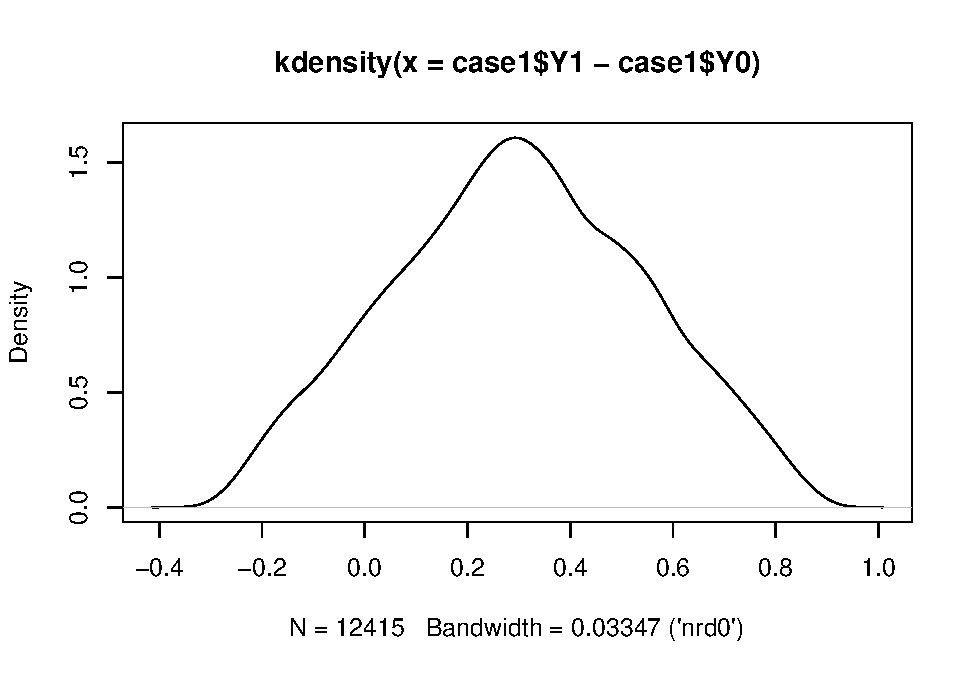
\includegraphics{Ogle_MicroMetricsAssignment_3_Q1_files/figure-latex/unnamed-chunk-10-1.pdf}

\begin{Shaded}
\begin{Highlighting}[]
\KeywordTok{plot}\NormalTok{(}\KeywordTok{kdensity}\NormalTok{(case1}\OperatorTok{$}\NormalTok{Y1[case1}\OperatorTok{$}\NormalTok{male}\OperatorTok{==}\DecValTok{1}\NormalTok{]}\OperatorTok{-}\NormalTok{case1}\OperatorTok{$}\NormalTok{Y0[case1}\OperatorTok{$}\NormalTok{male}\OperatorTok{==}\DecValTok{1}\NormalTok{]),}\DataTypeTok{col=}\StringTok{"blue"}\NormalTok{,}\DataTypeTok{main=}\StringTok{"Female Vs Male"}\NormalTok{)}
\KeywordTok{lines}\NormalTok{(}\KeywordTok{kdensity}\NormalTok{(case1}\OperatorTok{$}\NormalTok{Y1[case1}\OperatorTok{$}\NormalTok{male}\OperatorTok{==}\DecValTok{0}\NormalTok{]}\OperatorTok{-}\NormalTok{case1}\OperatorTok{$}\NormalTok{Y0[case1}\OperatorTok{$}\NormalTok{male}\OperatorTok{==}\DecValTok{0}\NormalTok{]),}\DataTypeTok{col=}\StringTok{"red"}\NormalTok{)}
\end{Highlighting}
\end{Shaded}

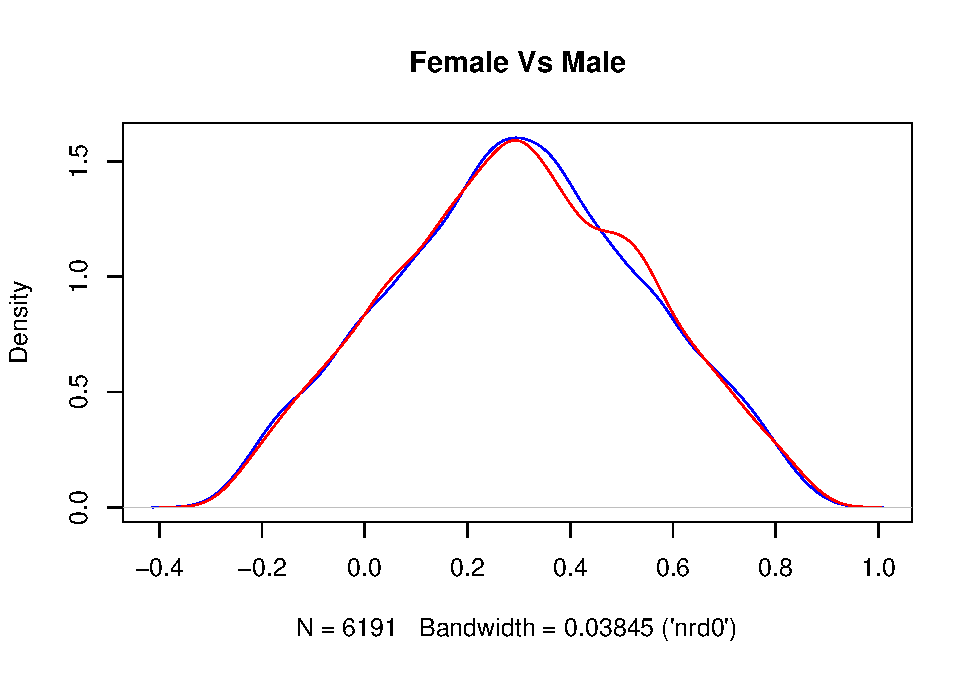
\includegraphics{Ogle_MicroMetricsAssignment_3_Q1_files/figure-latex/unnamed-chunk-10-2.pdf}

\begin{Shaded}
\begin{Highlighting}[]
\KeywordTok{plot}\NormalTok{(}\KeywordTok{kdensity}\NormalTok{(case1}\OperatorTok{$}\NormalTok{Y1[case1}\OperatorTok{$}\NormalTok{std}\OperatorTok{==}\DecValTok{3}\NormalTok{]}\OperatorTok{-}\NormalTok{case1}\OperatorTok{$}\NormalTok{Y0[case1}\OperatorTok{$}\NormalTok{std}\OperatorTok{==}\DecValTok{3}\NormalTok{]),}\DataTypeTok{col=}\StringTok{"blue"}\NormalTok{,}\DataTypeTok{main=}\StringTok{"3'rd vs 4th grade"}\NormalTok{)}
\KeywordTok{lines}\NormalTok{(}\KeywordTok{kdensity}\NormalTok{(case1}\OperatorTok{$}\NormalTok{Y1[case1}\OperatorTok{$}\NormalTok{std}\OperatorTok{==}\DecValTok{4}\NormalTok{]}\OperatorTok{-}\NormalTok{case1}\OperatorTok{$}\NormalTok{Y0[case1}\OperatorTok{$}\NormalTok{std}\OperatorTok{==}\DecValTok{4}\NormalTok{]),}\DataTypeTok{col=}\StringTok{"red"}\NormalTok{)}
\end{Highlighting}
\end{Shaded}

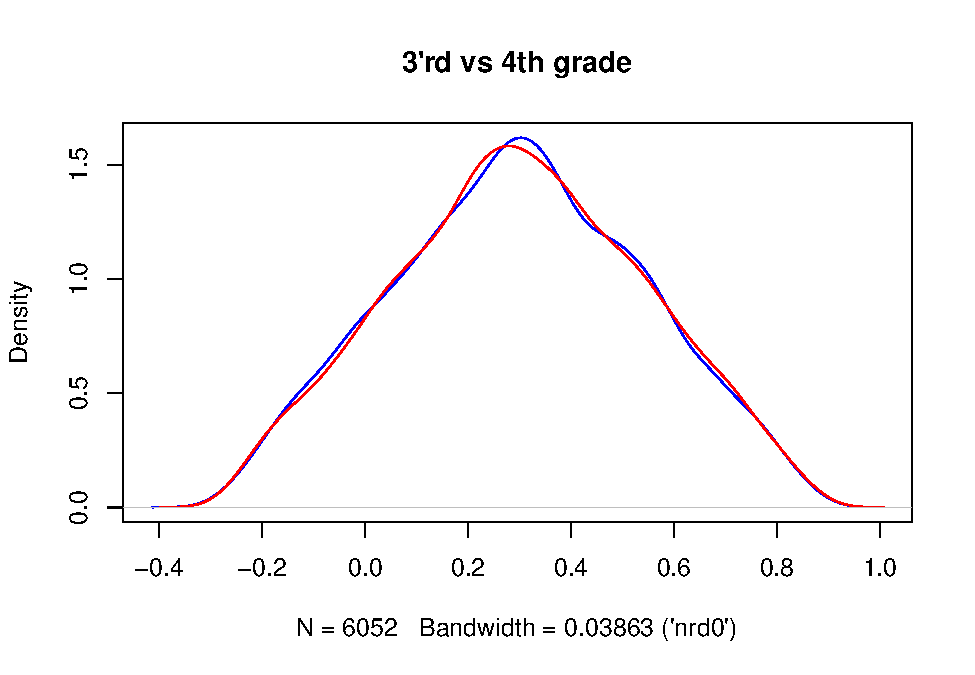
\includegraphics{Ogle_MicroMetricsAssignment_3_Q1_files/figure-latex/unnamed-chunk-10-3.pdf}

\begin{Shaded}
\begin{Highlighting}[]
\KeywordTok{plot}\NormalTok{(}\KeywordTok{kdensity}\NormalTok{(case1}\OperatorTok{$}\NormalTok{Y1[case1}\OperatorTok{$}\NormalTok{numstud}\OperatorTok{>=}\DecValTok{60}\NormalTok{]}\OperatorTok{-}\NormalTok{case1}\OperatorTok{$}\NormalTok{Y0[case1}\OperatorTok{$}\NormalTok{numstud}\OperatorTok{>=}\DecValTok{60}\NormalTok{]),}\DataTypeTok{col=}\StringTok{"blue"}\NormalTok{,}\DataTypeTok{main=}\StringTok{"NumStud"}\NormalTok{)}
\KeywordTok{lines}\NormalTok{(}\KeywordTok{kdensity}\NormalTok{(case1}\OperatorTok{$}\NormalTok{Y1[case1}\OperatorTok{$}\NormalTok{numstud}\OperatorTok{<}\DecValTok{60}\NormalTok{]}\OperatorTok{-}\NormalTok{case1}\OperatorTok{$}\NormalTok{Y0[case1}\OperatorTok{$}\NormalTok{numstud}\OperatorTok{<}\DecValTok{60}\NormalTok{]),}\DataTypeTok{col=}\StringTok{"red"}\NormalTok{)}
\end{Highlighting}
\end{Shaded}

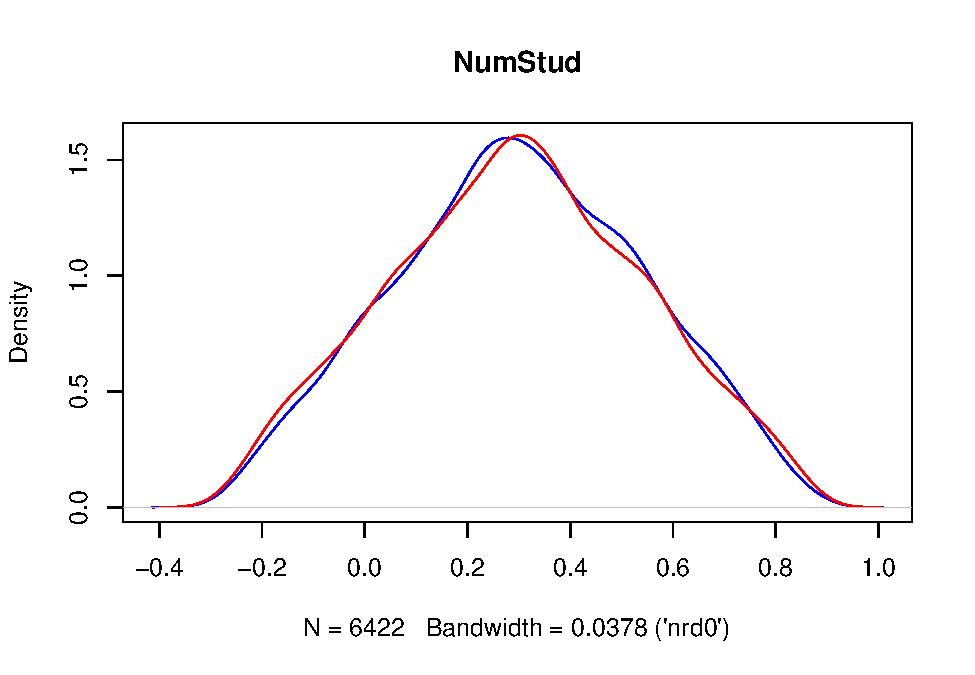
\includegraphics{Ogle_MicroMetricsAssignment_3_Q1_files/figure-latex/unnamed-chunk-10-4.pdf}
(l)

\begin{table}[H] \centering 
  \caption{Regression Results (l)} 
  \label{} 
\begin{tabular}{@{\extracolsep{5pt}}lcc} 
\\[-1.8ex]\hline 
\hline \\[-1.8ex] 
 & \multicolumn{2}{c}{\textit{Dependent variable:}} \\ 
\cline{2-3} 
\\[-1.8ex] & \multicolumn{2}{c}{treated} \\ 
 & Without Robust Std. Errors & With Robust Std. Errors \\ 
\\[-1.8ex] & (1) & (2)\\ 
\hline \\[-1.8ex] 
 std & $-$0.006 & $-$0.006 \\ 
  & (0.009) & (8.987e-03) \\ 
  & & \\ 
 male & $-$0.001 & $-$0.001 \\ 
  & (0.009) & (8.987e-03) \\ 
  & & \\ 
 numstud & 0.00002 & 0.00002 \\ 
  & (0.0002) & (1.728e-04) \\ 
  & & \\ 
 pre\_totnorm & $-$0.003 & $-$0.003 \\ 
  & (0.007) & (6.514e-03) \\ 
  & & \\ 
 income & $-$0.00001 & $-$0.00001 \\ 
  & (0.0002) & (1.559e-04) \\ 
  & & \\ 
 Constant & 0.520$^{***}$ & 0.520$^{***}$ \\ 
  & (0.041) & ( 4.057e-02 ) \\ 
  & & \\ 
\hline \\[-1.8ex] 
Observations & 12,415 & 12,415 \\ 
R$^{2}$ & 0.0001 & 0.0001 \\ 
Adjusted R$^{2}$ & $-$0.0003 & $-$0.0003 \\ 
Residual Std. Error (df = 12409) & 0.500 & 0.500 \\ 
F Statistic (df = 5; 12409) & 0.238 & 0.238 \\ 
\hline 
\hline \\[-1.8ex] 
\textit{Note:}  & \multicolumn{2}{r}{$^{*}$p$<$0.1; $^{**}$p$<$0.05; $^{***}$p$<$0.01} \\ 
\end{tabular} 
\end{table}

From our results it looks like there is balance between the treatment
group and the control. This is because most of the coefficients are very
close to 0. However, we know that few of the results are statistically
significant so we cannot be sure that the groups are balanced.

\begin{enumerate}
\def\labelenumi{(\alph{enumi})}
\setcounter{enumi}{12}
\item
\end{enumerate}

\begin{table}[H] \centering 
  \caption{Regression Results (l)} 
  \label{} 
\begin{tabular}{@{\extracolsep{5pt}}lc} 
\\[-1.8ex]\hline 
\hline \\[-1.8ex] 
 & \multicolumn{1}{c}{\textit{Dependent variable:}} \\ 
\cline{2-2} 
\\[-1.8ex] & Finalscore \\ 
\hline \\[-1.8ex] 
 treated & 0.047$^{***}$ \\ 
  & (0.004) \\ 
  & \\ 
 pre\_totnorm & 0.999$^{***}$ \\ 
  & (0.002) \\ 
  & \\ 
 Constant & $-$0.001 \\ 
  & (0.003) \\ 
  & \\ 
\hline \\[-1.8ex] 
Observations & 12,415 \\ 
R$^{2}$ & 0.942 \\ 
Adjusted R$^{2}$ & 0.942 \\ 
Residual Std. Error & 0.249 (df = 12412) \\ 
F Statistic & 101,181.400$^{***}$ (df = 2; 12412) \\ 
\hline 
\hline \\[-1.8ex] 
\textit{Note:}  & \multicolumn{1}{r}{$^{*}$p$<$0.1; $^{**}$p$<$0.05; $^{***}$p$<$0.01} \\ 
\end{tabular} 
\end{table}

The model we regress comes from regressing our final outcome score on
the treatment and then the pretest score. We need MLR.4 which is the
zero conditional mean to hold for consistency and causality to be
considered. I think that MLR.4 is not credible. There are many different
variables that are in the error term and are correlated with the
independent variables. For example, how much the student studies
indepentely of the study, how much help the child has when studying
outside the school, the mental and physical health of the student. We
would want to control for these variables to make a causal conclusion.

\begin{enumerate}
\def\labelenumi{(\alph{enumi})}
\setcounter{enumi}{13}
\item
\end{enumerate}

We can improve the precision of the estimator by performing a BP test to
test for heteroskedasticity. Then we can account for the
heteroskedasticity by using robust standard errors to make our results
more meaningful.

The results of our BP test yield the following results: BP = 2294, df =
2, p-value \textless{} 2.2e-16

Because the p-value is greater than 0.05 we can reject our null
hypothesis of homoskedasticity. We can conclude that the model is
heteroskedastic and we need use Robust Standard Errors to make our model
more meaningful and precise. However, this is one way to make the model
more precise to view these standard error look to the table.

\begin{table}[!htbp] \centering 
  \caption{Regression Results (n)} 
  \label{} 
\begin{tabular}{@{\extracolsep{5pt}}lc} 
\\[-1.8ex]\hline 
\hline \\[-1.8ex] 
 & \multicolumn{1}{c}{\textit{Dependent variable:}} \\ 
\cline{2-2} 
\\[-1.8ex] & Finalscore \\ 
\hline \\[-1.8ex] 
 treated & 0.047$^{***}$ \\ 
  & (0.0044686) \\ 
  & \\ 
 pre\_totnorm & 0.999$^{***}$ \\ 
  & (0.0022304) \\ 
  & \\ 
 Constant & $-$0.001 \\ 
  & (0.0022013) \\ 
  & \\ 
\hline \\[-1.8ex] 
Observations & 12,415 \\ 
R$^{2}$ & 0.942 \\ 
Adjusted R$^{2}$ & 0.942 \\ 
Residual Std. Error & 0.249 (df = 12412) \\ 
F Statistic & 101,181.400$^{***}$ (df = 2; 12412) \\ 
\hline 
\hline \\[-1.8ex] 
\textit{Note:}  & \multicolumn{1}{r}{$^{*}$p$<$0.1; $^{**}$p$<$0.05; $^{***}$p$<$0.01} \\ 
\end{tabular} 
\end{table}

\begin{enumerate}
\def\labelenumi{(\alph{enumi})}
\setcounter{enumi}{14}
\item
\end{enumerate}

\begin{table}[H] \centering 
  \caption{Regression Results (o)} 
  \label{} 
\begin{tabular}{@{\extracolsep{5pt}}lD{.}{.}{-3} D{.}{.}{-3} D{.}{.}{-3} } 
\\[-1.8ex]\hline 
\hline \\[-1.8ex] 
 & \multicolumn{3}{c}{\textit{Dependent variable:}} \\ 
\cline{2-4} 
 & \multicolumn{1}{c}{Final Scores} & \multicolumn{1}{c}{High Income} & \multicolumn{1}{c}{Low Income} \\ 
\\[-1.8ex] & \multicolumn{1}{c}{(1)} & \multicolumn{1}{c}{(2)} & \multicolumn{1}{c}{(3)}\\ 
\hline \\[-1.8ex] 
 treated & 0.047^{***} & -0.774 & 0.303 \\ 
  & (0.004) & (0.528) & (0.493) \\ 
  & & & \\ 
 pre\_totnorm & 0.999^{***} & 17.761^{***} & 14.862^{***} \\ 
  & (0.002) & (0.257) & (0.403) \\ 
  & & & \\ 
 Constant & -0.001 & 175.097^{***} & 124.743^{***} \\ 
  & (0.003) & (0.403) & (0.404) \\ 
  & & & \\ 
\hline \\[-1.8ex] 
Observations & \multicolumn{1}{c}{12,415} & \multicolumn{1}{c}{6,104} & \multicolumn{1}{c}{6,311} \\ 
R$^{2}$ & \multicolumn{1}{c}{0.942} & \multicolumn{1}{c}{0.439} & \multicolumn{1}{c}{0.177} \\ 
Adjusted R$^{2}$ & \multicolumn{1}{c}{0.942} & \multicolumn{1}{c}{0.439} & \multicolumn{1}{c}{0.177} \\ 
Residual Std. Error & \multicolumn{1}{c}{0.249 (df = 12412)} & \multicolumn{1}{c}{20.623 (df = 6101)} & \multicolumn{1}{c}{19.586 (df = 6308)} \\ 
F Statistic & \multicolumn{1}{c}{101,181.400$^{***}$ (df = 2; 12412)} & \multicolumn{1}{c}{2,385.462$^{***}$ (df = 2; 6101)} & \multicolumn{1}{c}{680.199$^{***}$ (df = 2; 6308)} \\ 
\hline 
\hline \\[-1.8ex] 
\textit{Note:}  & \multicolumn{3}{l}{$^{*}$p$<$0.1; $^{**}$p$<$0.05; $^{***}$p$<$0.01} \\ 
 & \multicolumn{3}{l}{Standard errors in parentheses} \\ 
\end{tabular} 
\end{table}

\begin{table}[H] \centering 
  \caption{Regression Results (o)} 
  \label{} 
\begin{tabular}{@{\extracolsep{5pt}}lD{.}{.}{-3} D{.}{.}{-3} D{.}{.}{-3} } 
\\[-1.8ex]\hline 
\hline \\[-1.8ex] 
 & \multicolumn{3}{c}{\textit{Dependent variable:}} \\ 
\cline{2-4} 
 & \multicolumn{1}{c}{High Students} & \multicolumn{1}{c}{Low Students} & \multicolumn{1}{c}{Male} \\ 
\\[-1.8ex] & \multicolumn{1}{c}{(1)} & \multicolumn{1}{c}{(2)} & \multicolumn{1}{c}{(3)}\\ 
\hline \\[-1.8ex] 
 treated & -0.338 & 0.018 & -0.001 \\ 
  & (0.484) & (0.303) & (0.009) \\ 
  & & & \\ 
 pre\_totnorm & 1.289^{***} & -0.090 & -0.022^{***} \\ 
  & (0.246) & (0.149) & (0.004) \\ 
  & & & \\ 
 Constant & 85.067^{***} & 43.166^{***} & 0.500^{***} \\ 
  & (0.343) & (0.214) & (0.006) \\ 
  & & & \\ 
\hline \\[-1.8ex] 
Observations & \multicolumn{1}{c}{5,876} & \multicolumn{1}{c}{6,539} & \multicolumn{1}{c}{12,415} \\ 
R$^{2}$ & \multicolumn{1}{c}{0.005} & \multicolumn{1}{c}{0.0001} & \multicolumn{1}{c}{0.002} \\ 
Adjusted R$^{2}$ & \multicolumn{1}{c}{0.004} & \multicolumn{1}{c}{-0.0002} & \multicolumn{1}{c}{0.002} \\ 
Residual Std. Error & \multicolumn{1}{c}{18.556 (df = 5873)} & \multicolumn{1}{c}{12.259 (df = 6536)} & \multicolumn{1}{c}{0.500 (df = 12412)} \\ 
F Statistic & \multicolumn{1}{c}{13.975$^{***}$ (df = 2; 5873)} & \multicolumn{1}{c}{0.183 (df = 2; 6536)} & \multicolumn{1}{c}{12.068$^{***}$ (df = 2; 12412)} \\ 
\hline 
\hline \\[-1.8ex] 
\textit{Note:}  & \multicolumn{3}{l}{$^{*}$p$<$0.1; $^{**}$p$<$0.05; $^{***}$p$<$0.01} \\ 
 & \multicolumn{3}{l}{Standard errors in parentheses} \\ 
\end{tabular} 
\end{table}

\begin{enumerate}
\def\labelenumi{(\alph{enumi})}
\setcounter{enumi}{15}
\item
\end{enumerate}

\begin{Shaded}
\begin{Highlighting}[]
\KeywordTok{plot}\NormalTok{(}\KeywordTok{kdensity}\NormalTok{(case2}\OperatorTok{$}\NormalTok{Y1}\OperatorTok{-}\NormalTok{case2}\OperatorTok{$}\NormalTok{Y0))}
\end{Highlighting}
\end{Shaded}

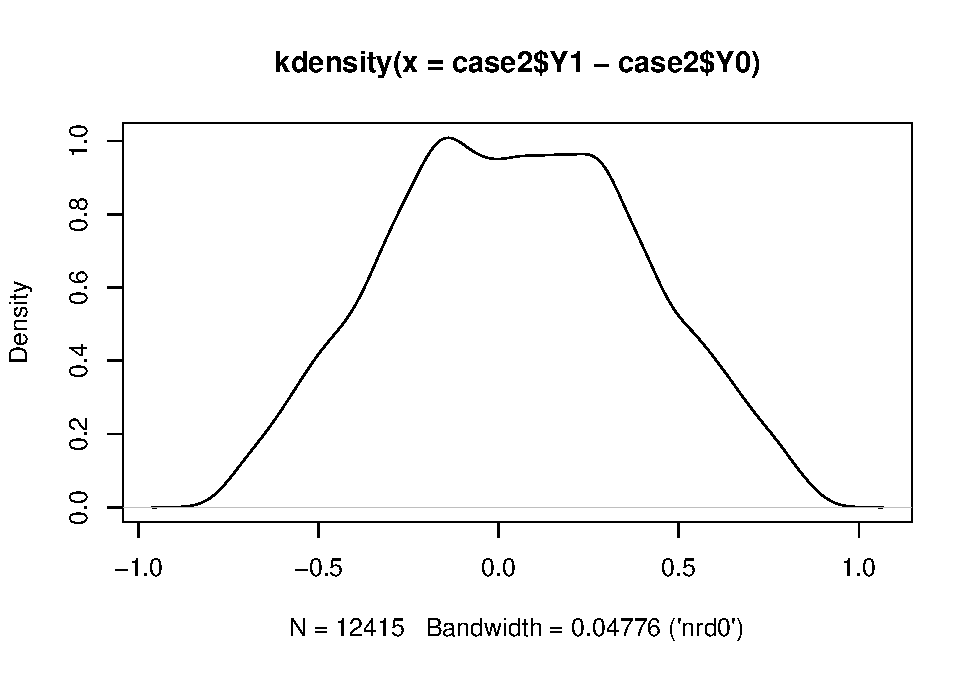
\includegraphics{Ogle_MicroMetricsAssignment_3_Q1_files/figure-latex/unnamed-chunk-15-1.pdf}

\begin{Shaded}
\begin{Highlighting}[]
\KeywordTok{plot}\NormalTok{(}\KeywordTok{kdensity}\NormalTok{(case2}\OperatorTok{$}\NormalTok{Y1[case2}\OperatorTok{$}\NormalTok{male}\OperatorTok{==}\DecValTok{1}\NormalTok{]}\OperatorTok{-}\NormalTok{case2}\OperatorTok{$}\NormalTok{Y0[case2}\OperatorTok{$}\NormalTok{male}\OperatorTok{==}\DecValTok{1}\NormalTok{]),}\DataTypeTok{col=}\StringTok{"blue"}\NormalTok{,}\DataTypeTok{main=}\StringTok{"Female Vs Male"}\NormalTok{)}
\KeywordTok{lines}\NormalTok{(}\KeywordTok{kdensity}\NormalTok{(case2}\OperatorTok{$}\NormalTok{Y1[case2}\OperatorTok{$}\NormalTok{male}\OperatorTok{==}\DecValTok{0}\NormalTok{]}\OperatorTok{-}\NormalTok{case2}\OperatorTok{$}\NormalTok{Y0[case2}\OperatorTok{$}\NormalTok{male}\OperatorTok{==}\DecValTok{0}\NormalTok{]),}\DataTypeTok{col=}\StringTok{"red"}\NormalTok{)}
\end{Highlighting}
\end{Shaded}

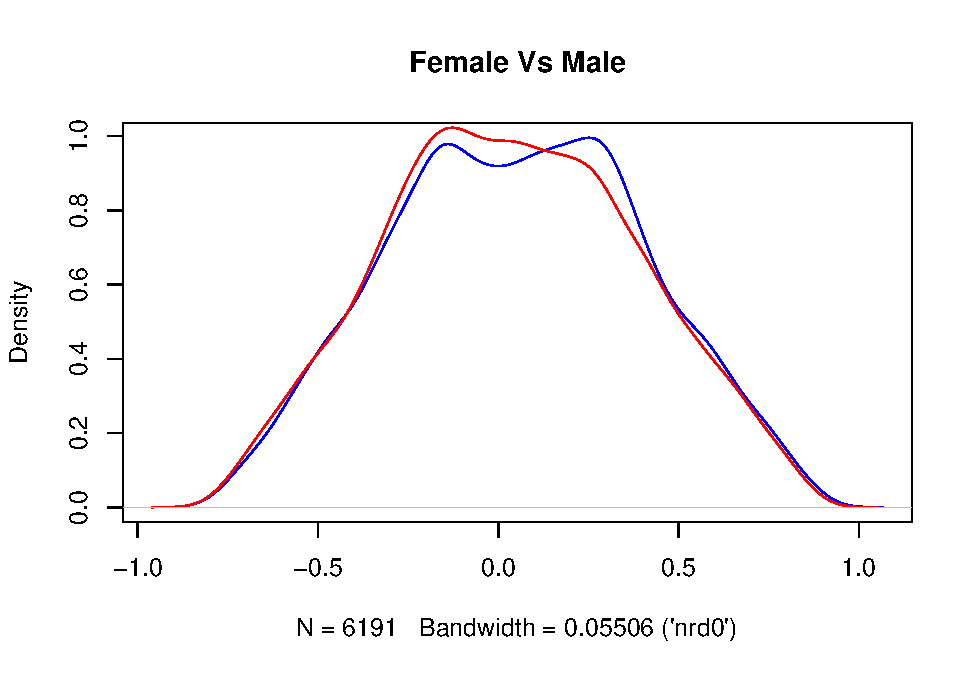
\includegraphics{Ogle_MicroMetricsAssignment_3_Q1_files/figure-latex/unnamed-chunk-15-2.pdf}

\begin{Shaded}
\begin{Highlighting}[]
\KeywordTok{plot}\NormalTok{(}\KeywordTok{kdensity}\NormalTok{(case2}\OperatorTok{$}\NormalTok{Y1[case2}\OperatorTok{$}\NormalTok{std}\OperatorTok{==}\DecValTok{3}\NormalTok{]}\OperatorTok{-}\NormalTok{case2}\OperatorTok{$}\NormalTok{Y0[case2}\OperatorTok{$}\NormalTok{std}\OperatorTok{==}\DecValTok{3}\NormalTok{]),}\DataTypeTok{col=}\StringTok{"blue"}\NormalTok{,}\DataTypeTok{main=}\StringTok{"3'rd vs 4th grade"}\NormalTok{)}
\KeywordTok{lines}\NormalTok{(}\KeywordTok{kdensity}\NormalTok{(case2}\OperatorTok{$}\NormalTok{Y1[case2}\OperatorTok{$}\NormalTok{std}\OperatorTok{==}\DecValTok{4}\NormalTok{]}\OperatorTok{-}\NormalTok{case2}\OperatorTok{$}\NormalTok{Y0[case2}\OperatorTok{$}\NormalTok{std}\OperatorTok{==}\DecValTok{4}\NormalTok{]),}\DataTypeTok{col=}\StringTok{"red"}\NormalTok{)}
\end{Highlighting}
\end{Shaded}

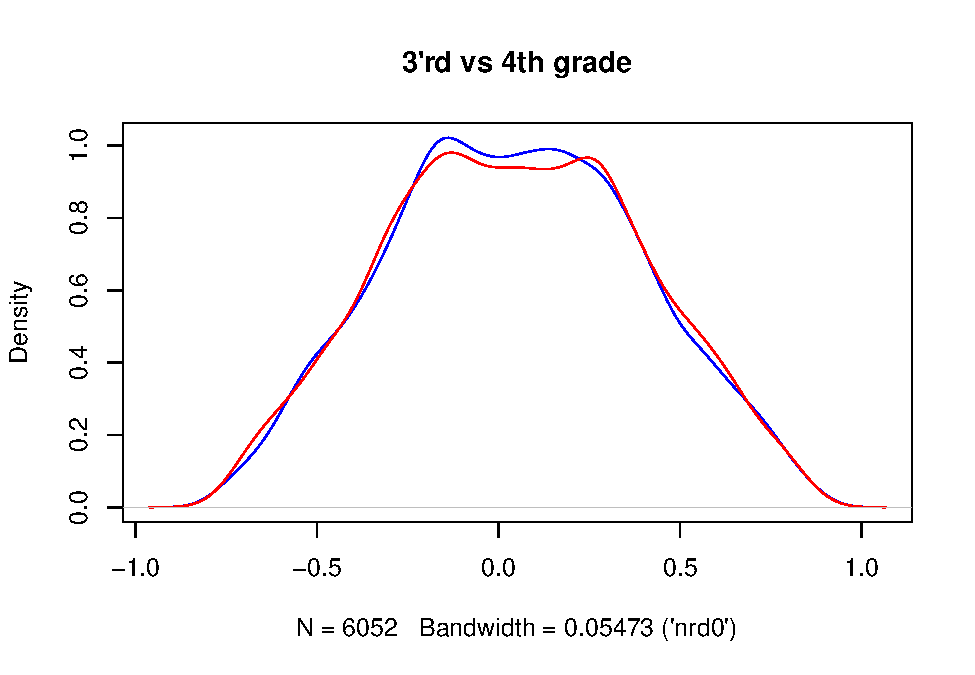
\includegraphics{Ogle_MicroMetricsAssignment_3_Q1_files/figure-latex/unnamed-chunk-15-3.pdf}

\begin{Shaded}
\begin{Highlighting}[]
\KeywordTok{plot}\NormalTok{(}\KeywordTok{kdensity}\NormalTok{(case2}\OperatorTok{$}\NormalTok{Y1[case2}\OperatorTok{$}\NormalTok{numstud}\OperatorTok{>=}\DecValTok{60}\NormalTok{]}\OperatorTok{-}\NormalTok{case2}\OperatorTok{$}\NormalTok{Y0[case2}\OperatorTok{$}\NormalTok{numstud}\OperatorTok{>=}\DecValTok{60}\NormalTok{]),}\DataTypeTok{col=}\StringTok{"blue"}\NormalTok{,}\DataTypeTok{main=}\StringTok{"NumStud"}\NormalTok{)}
\KeywordTok{lines}\NormalTok{(}\KeywordTok{kdensity}\NormalTok{(case2}\OperatorTok{$}\NormalTok{Y1[case2}\OperatorTok{$}\NormalTok{numstud}\OperatorTok{<}\DecValTok{60}\NormalTok{]}\OperatorTok{-}\NormalTok{case2}\OperatorTok{$}\NormalTok{Y0[case2}\OperatorTok{$}\NormalTok{numstud}\OperatorTok{<}\DecValTok{60}\NormalTok{]),}\DataTypeTok{col=}\StringTok{"red"}\NormalTok{)}
\end{Highlighting}
\end{Shaded}

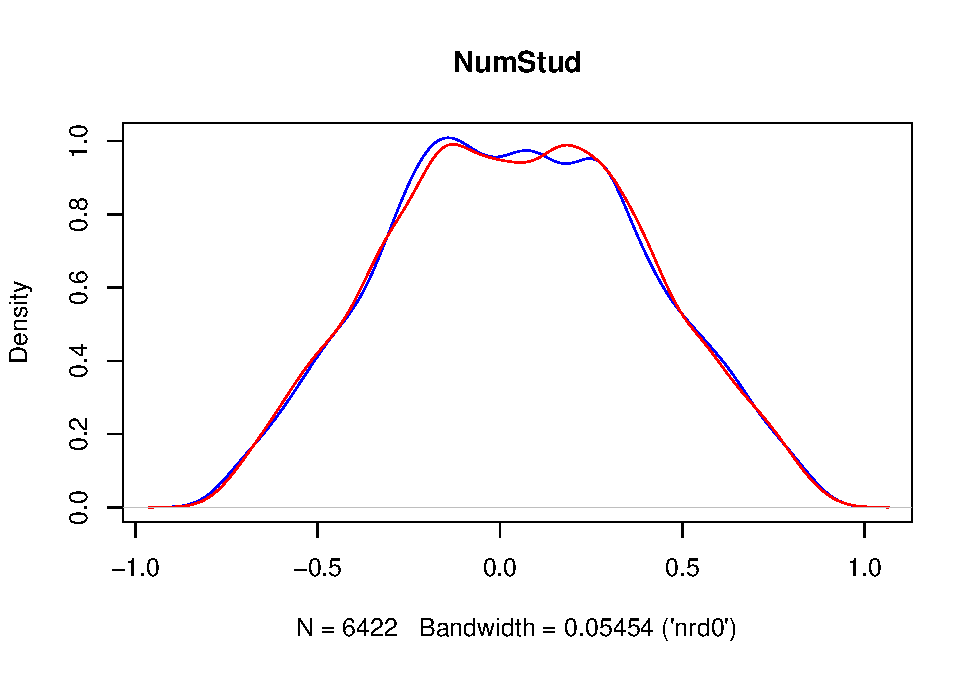
\includegraphics{Ogle_MicroMetricsAssignment_3_Q1_files/figure-latex/unnamed-chunk-15-4.pdf}

\begin{enumerate}
\def\labelenumi{(\alph{enumi})}
\setcounter{enumi}{16}
\item
\end{enumerate}

\begin{Shaded}
\begin{Highlighting}[]
\KeywordTok{hist}\NormalTok{(case2}\OperatorTok{$}\NormalTok{Y1[case2}\OperatorTok{$}\NormalTok{side }\OperatorTok{==}\StringTok{ }\DecValTok{1}\NormalTok{] }\OperatorTok{-}\StringTok{ }\NormalTok{case2}\OperatorTok{$}\NormalTok{Y0[case2}\OperatorTok{$}\NormalTok{side }\OperatorTok{==}\StringTok{ }\DecValTok{1}\NormalTok{], }\DataTypeTok{main =} \StringTok{"Average Treatment Effect by Side"}\NormalTok{,}
    \DataTypeTok{col =} \KeywordTok{rgb}\NormalTok{(}\DecValTok{1}\NormalTok{, }\DecValTok{0}\NormalTok{, }\DecValTok{0}\NormalTok{, }\FloatTok{.5}\NormalTok{),}
    \DataTypeTok{xlab =} \StringTok{"Final Score"}\NormalTok{,}
    \DataTypeTok{ylab =} \StringTok{"Frequency"}\NormalTok{,}
    \DataTypeTok{xlim =} \KeywordTok{c}\NormalTok{(}\OperatorTok{-}\DecValTok{1}\NormalTok{, }\DecValTok{1}\NormalTok{),}
    \DataTypeTok{ylim =} \KeywordTok{c}\NormalTok{(}\DecValTok{0}\NormalTok{, }\DecValTok{250}\NormalTok{),}
    \DataTypeTok{breaks =} \DecValTok{50}\NormalTok{)}
\KeywordTok{hist}\NormalTok{(case2}\OperatorTok{$}\NormalTok{Y1[case2}\OperatorTok{$}\NormalTok{side }\OperatorTok{==}\StringTok{ }\DecValTok{0}\NormalTok{] }\OperatorTok{-}\StringTok{ }\NormalTok{case2}\OperatorTok{$}\NormalTok{Y0[case2}\OperatorTok{$}\NormalTok{side }\OperatorTok{==}\StringTok{ }\DecValTok{0}\NormalTok{],}
    \DataTypeTok{col =} \KeywordTok{rgb}\NormalTok{(}\DecValTok{0}\NormalTok{, }\DecValTok{0}\NormalTok{, }\DecValTok{1}\NormalTok{, }\FloatTok{.5}\NormalTok{),}
    \DataTypeTok{breaks =} \DecValTok{50}\NormalTok{,}
    \DataTypeTok{add =} \OtherTok{TRUE}\NormalTok{)}
\end{Highlighting}
\end{Shaded}

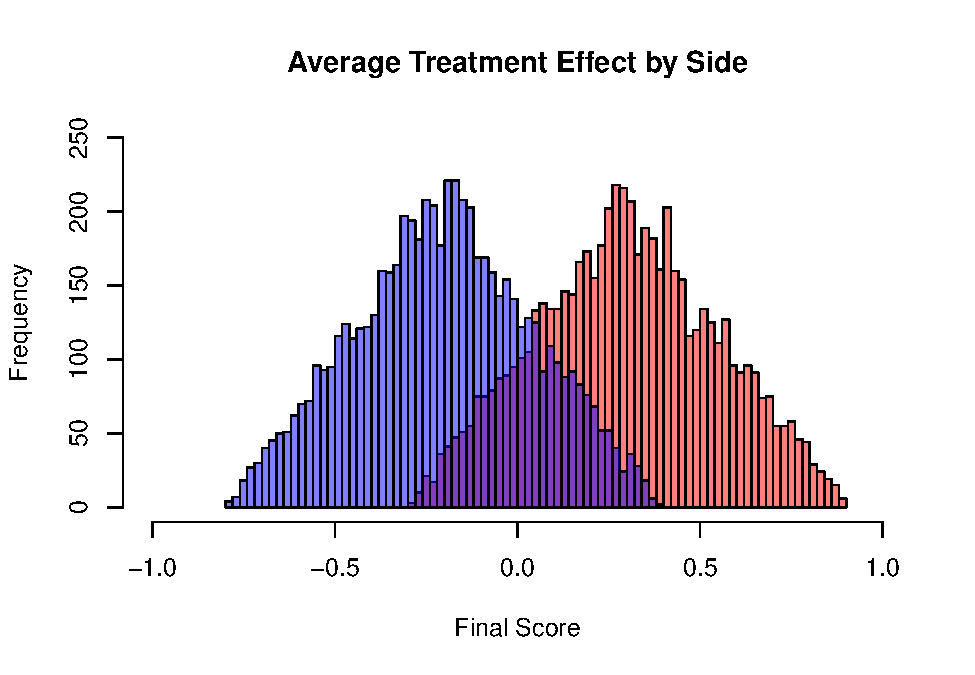
\includegraphics{Ogle_MicroMetricsAssignment_3_Q1_files/figure-latex/unnamed-chunk-16-1.pdf}

The red is a presence of side and red is where side is not present.

\begin{table}[H] \centering 
  \caption{Regression Results (q)} 
  \label{} 
\begin{tabular}{@{\extracolsep{5pt}}lD{.}{.}{-3} } 
\\[-1.8ex]\hline 
\hline \\[-1.8ex] 
 & \multicolumn{1}{c}{\textit{Dependent variable:}} \\ 
\cline{2-2} 
\\[-1.8ex] & \multicolumn{1}{c}{Finalscore} \\ 
\hline \\[-1.8ex] 
 std & -0.005 \\ 
  & (0.004) \\ 
  & \\ 
 male & -0.0004 \\ 
  & (0.004) \\ 
  & \\ 
 numstud & -0.0001 \\ 
  & (0.0001) \\ 
  & \\ 
 pre\_totnorm & 0.998^{***} \\ 
  & (0.003) \\ 
  & \\ 
 income & 0.00001 \\ 
  & (0.0001) \\ 
  & \\ 
 treated & 0.049^{***} \\ 
  & (0.004) \\ 
  & \\ 
 side & 0.252^{***} \\ 
  & (0.004) \\ 
  & \\ 
 Constant & -0.106^{***} \\ 
  & (0.018) \\ 
  & \\ 
\hline \\[-1.8ex] 
Observations & \multicolumn{1}{c}{12,415} \\ 
R$^{2}$ & \multicolumn{1}{c}{0.957} \\ 
Adjusted R$^{2}$ & \multicolumn{1}{c}{0.957} \\ 
Residual Std. Error & \multicolumn{1}{c}{0.214 (df = 12407)} \\ 
F Statistic & \multicolumn{1}{c}{39,490.520$^{***}$ (df = 7; 12407)} \\ 
\hline 
\hline \\[-1.8ex] 
\textit{Note:}  & \multicolumn{1}{l}{$^{*}$p$<$0.1; $^{**}$p$<$0.05; $^{***}$p$<$0.01} \\ 
 & \multicolumn{1}{l}{Standard errors in parentheses} \\ 
\end{tabular} 
\end{table}

As we can see in the model above, the addition of side greatly increase
the R-squared value and adjusted R-squared value. Because we did not see
a significant change in our coefficeints and we saw this increase of fit
to our regression model we would want to keep side included in our
model.

\begin{enumerate}
\def\labelenumi{(\alph{enumi})}
\setcounter{enumi}{17}
\item
\end{enumerate}

The average treament effect does not mean much. As we see from the graph
in a the effect of the treatment is not homogeneous with respect to
side. If side is present, than the average effect of the treatment is
shown to be significantly greater, because students, on average, achieve
much higher final scores. Compare this to when side is not present,
where the average effect of the treatment is shown to be significantly
less, because students, on average, achieve much lower final scores. If
side were = to wealth it would follow these previous results. If
students have more resources in general then they are more likely to be
a good student because they can purchase tutors and better equipment and
have more time to study and not work.

\begin{enumerate}
\def\labelenumi{(\alph{enumi})}
\setcounter{enumi}{18}
\item
\end{enumerate}

\begin{table}[H] \centering 
  \caption{Regression Results (s)} 
  \label{} 
\begin{tabular}{@{\extracolsep{5pt}}lD{.}{.}{-3} } 
\\[-1.8ex]\hline 
\hline \\[-1.8ex] 
 & \multicolumn{1}{c}{\textit{Dependent variable:}} \\ 
\cline{2-2} 
\\[-1.8ex] & \multicolumn{1}{c}{Finalscore} \\ 
\hline \\[-1.8ex] 
 std & -0.005 \\ 
  & (0.004) \\ 
  & \\ 
 male & -0.0004 \\ 
  & (0.004) \\ 
  & \\ 
 numstud & -0.0001 \\ 
  & (0.0001) \\ 
  & \\ 
 pre\_totnorm & 0.998^{***} \\ 
  & (0.003) \\ 
  & \\ 
 income & 0.00001 \\ 
  & (0.0001) \\ 
  & \\ 
 treated & 0.049^{***} \\ 
  & (0.004) \\ 
  & \\ 
 side & 0.252^{***} \\ 
  & (0.004) \\ 
  & \\ 
 Constant & -0.106^{***} \\ 
  & (0.018) \\ 
  & \\ 
\hline \\[-1.8ex] 
Observations & \multicolumn{1}{c}{12,415} \\ 
R$^{2}$ & \multicolumn{1}{c}{0.957} \\ 
Adjusted R$^{2}$ & \multicolumn{1}{c}{0.957} \\ 
Residual Std. Error & \multicolumn{1}{c}{0.214 (df = 12407)} \\ 
F Statistic & \multicolumn{1}{c}{39,490.520$^{***}$ (df = 7; 12407)} \\ 
\hline 
\hline \\[-1.8ex] 
\textit{Note:}  & \multicolumn{1}{l}{$^{*}$p$<$0.1; $^{**}$p$<$0.05; $^{***}$p$<$0.01} \\ 
 & \multicolumn{1}{l}{Standard errors in parentheses} \\ 
\end{tabular} 
\end{table}

We can conclude that the two groups are balanced because all of the
coefficients from this regression are close to 0 and pretest treated and
side are all statistically significant values.

Randomization is not successful. In the regression on assigned
treatment, the coefficient for normalized pre test score was not
obtained with statistical significance. Although the assignment to
treatment may have been random, randomization was not successful. This
was due to the significant estimate for the coefficient of the
normalized pre-test score variable.

\begin{enumerate}
\def\labelenumi{(\alph{enumi})}
\setcounter{enumi}{19}
\item
\end{enumerate}

\begin{table}[H] \centering 
  \caption{Regression Results (t)} 
  \label{} 
\begin{tabular}{@{\extracolsep{5pt}}lD{.}{.}{-3} } 
\\[-1.8ex]\hline 
\hline \\[-1.8ex] 
 & \multicolumn{1}{c}{\textit{Dependent variable:}} \\ 
\cline{2-2} 
\\[-1.8ex] & \multicolumn{1}{c}{(TreatmentGroup - treated)} \\ 
\hline \\[-1.8ex] 
 std & -0.008 \\ 
  & (0.006) \\ 
  & \\ 
 male & 0.007 \\ 
  & (0.006) \\ 
  & \\ 
 numstud & 0.0002 \\ 
  & (0.0001) \\ 
  & \\ 
 pre\_totnorm & 0.014^{***} \\ 
  & (0.005) \\ 
  & \\ 
 income & -0.002^{***} \\ 
  & (0.0001) \\ 
  & \\ 
 Constant & 0.490^{***} \\ 
  & (0.029) \\ 
  & \\ 
\hline \\[-1.8ex] 
Observations & \multicolumn{1}{c}{12,415} \\ 
R$^{2}$ & \multicolumn{1}{c}{0.049} \\ 
Adjusted R$^{2}$ & \multicolumn{1}{c}{0.049} \\ 
Residual Std. Error & \multicolumn{1}{c}{0.352 (df = 12409)} \\ 
F Statistic & \multicolumn{1}{c}{129.166$^{***}$ (df = 5; 12409)} \\ 
\hline 
\hline \\[-1.8ex] 
\textit{Note:}  & \multicolumn{1}{l}{$^{*}$p$<$0.1; $^{**}$p$<$0.05; $^{***}$p$<$0.01} \\ 
 & \multicolumn{1}{l}{Standard errors in parentheses} \\ 
\end{tabular} 
\end{table}

Our coefficients here represent the likelihood or probability that
someone will dropout of school and in effect the treatment or control
group. We can see that a higher pretest scores lead to a higher
likelihood that the student will drop out. Conversely higher income
means that the student is less likely to drop out.

\begin{enumerate}
\def\labelenumi{(\alph{enumi})}
\setcounter{enumi}{20}
\item
\end{enumerate}

When we find the mean final score for the students who were treated we
get 0.4668035 and when we get the mean final score for no assigned
treatment group we get 0.02937351. We get ITT = 0.4668035 - 0.02937351 =
0.43743. Knowing the ITT coefficient is 0.43743 tells us and other
policy makers that the average effect of assigning treatment is 0.43743.

\begin{enumerate}
\def\labelenumi{(\alph{enumi})}
\setcounter{enumi}{21}
\item
\end{enumerate}

\begin{table}[H] \centering 
  \caption{Regression Results (v)} 
  \label{} 
\begin{tabular}{@{\extracolsep{5pt}}lD{.}{.}{-3} D{.}{.}{-3} } 
\\[-1.8ex]\hline 
\hline \\[-1.8ex] 
 & \multicolumn{2}{c}{\textit{Dependent variable:}} \\ 
\cline{2-3} 
\\[-1.8ex] & \multicolumn{2}{c}{Finalscore} \\ 
\\[-1.8ex] & \multicolumn{1}{c}{(1)} & \multicolumn{1}{c}{(2)}\\ 
\hline \\[-1.8ex] 
 treated & 0.516^{***} &  \\ 
  & (0.019) &  \\ 
  & & \\ 
 pre\_totnorm &  & 1.015^{***} \\ 
  &  & (0.002) \\ 
  & & \\ 
 Constant & -0.049^{***} & 0.103^{***} \\ 
  & (0.011) & (0.002) \\ 
  & & \\ 
\hline \\[-1.8ex] 
Observations & \multicolumn{1}{c}{12,415} & \multicolumn{1}{c}{12,415} \\ 
R$^{2}$ & \multicolumn{1}{c}{0.055} & \multicolumn{1}{c}{0.954} \\ 
Adjusted R$^{2}$ & \multicolumn{1}{c}{0.055} & \multicolumn{1}{c}{0.954} \\ 
Residual Std. Error (df = 12413) & \multicolumn{1}{c}{1.015} & \multicolumn{1}{c}{0.224} \\ 
F Statistic (df = 1; 12413) & \multicolumn{1}{c}{729.238$^{***}$} & \multicolumn{1}{c}{258,009.200$^{***}$} \\ 
\hline 
\hline \\[-1.8ex] 
\textit{Note:}  & \multicolumn{2}{l}{$^{*}$p$<$0.1; $^{**}$p$<$0.05; $^{***}$p$<$0.01} \\ 
 & \multicolumn{2}{l}{Standard errors in parentheses} \\ 
\end{tabular} 
\end{table}

No our estimated treatment effect is biased we already know that there
is attrition students are dropping out of the program. There is
attrition bias. Additionally, MLR.4 is not very credible here either. In
order for the zero conditional mean assumption to hold there must be no
variables in the error term that are correlated with the independent
variables. To prove this we only need to perform a simple regression of
Final Scores on pretest normalized scores to see that they are
correlated. If this is the case then there must be variales in the error
term that are correlated with pretest scores.

\begin{enumerate}
\def\labelenumi{(\alph{enumi})}
\setcounter{enumi}{24}
\item
\end{enumerate}

\begin{Shaded}
\begin{Highlighting}[]
\NormalTok{case3_y <-}\StringTok{ }\KeywordTok{subset}\NormalTok{(case3, TreatmentGroup }\OperatorTok{==}\StringTok{ }\DecValTok{1}\NormalTok{)}
\NormalTok{case3_y <-}\StringTok{ }\KeywordTok{subset}\NormalTok{(case3_y, treated }\OperatorTok{==}\StringTok{ }\DecValTok{1}\NormalTok{)}

\KeywordTok{hist}\NormalTok{(case3_y}\OperatorTok{$}\NormalTok{Y1 }\OperatorTok{-}\StringTok{ }\NormalTok{case3_y}\OperatorTok{$}\NormalTok{Y0,}
    \DataTypeTok{col =} \KeywordTok{rgb}\NormalTok{(}\DecValTok{1}\NormalTok{, }\DecValTok{0}\NormalTok{, }\DecValTok{0}\NormalTok{, }\FloatTok{.5}\NormalTok{),}
    \DataTypeTok{xlim =} \KeywordTok{c}\NormalTok{(}\OperatorTok{-}\DecValTok{1}\NormalTok{, }\DecValTok{1}\NormalTok{),}
    \DataTypeTok{ylim =} \KeywordTok{c}\NormalTok{(}\DecValTok{0}\NormalTok{, }\DecValTok{200}\NormalTok{),}
    \DataTypeTok{breaks =} \DecValTok{50}\NormalTok{)}

\NormalTok{case3_y <-}\StringTok{ }\KeywordTok{subset}\NormalTok{(case3, TreatmentGroup }\OperatorTok{==}\StringTok{ }\DecValTok{1}\NormalTok{)}
\NormalTok{case3_y <-}\StringTok{ }\KeywordTok{subset}\NormalTok{(case3_y, treated }\OperatorTok{==}\StringTok{ }\DecValTok{0}\NormalTok{)}
\KeywordTok{hist}\NormalTok{(case3_y}\OperatorTok{$}\NormalTok{Y1 }\OperatorTok{-}\StringTok{ }\NormalTok{case3_y}\OperatorTok{$}\NormalTok{Y0,}
    \DataTypeTok{col =} \KeywordTok{rgb}\NormalTok{(}\DecValTok{0}\NormalTok{, }\DecValTok{0}\NormalTok{, }\DecValTok{1}\NormalTok{, }\FloatTok{.5}\NormalTok{),}
    \DataTypeTok{breaks =} \DecValTok{50}\NormalTok{,}
    \DataTypeTok{add =} \OtherTok{TRUE}\NormalTok{)}
\end{Highlighting}
\end{Shaded}

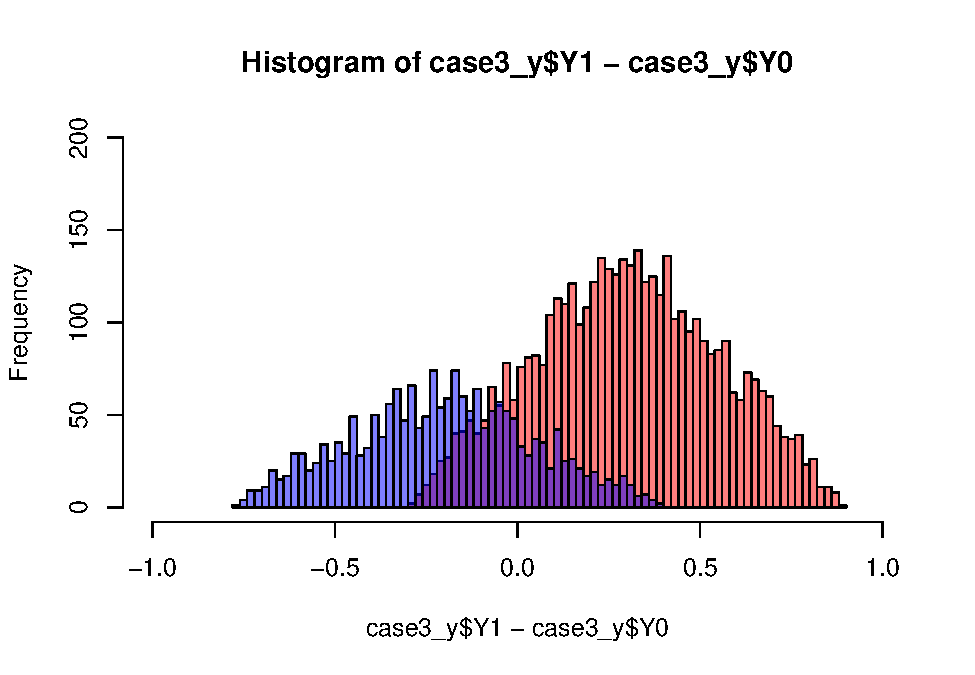
\includegraphics{Ogle_MicroMetricsAssignment_3_Q1_files/figure-latex/unnamed-chunk-22-1.pdf}

The blue are the students who dropped out the red are the students who
were eventually treated. Those that were eventually treated by the
treatment had better educational outcomes than those who dropped out.
These results are not consistent with rationality or rational
individuals. For example all rational students want to do well in school
and improve there scores on standardized tests so that they can improve
their knowledge and get a better higher paying job when they are older.
However, children and students are not all equally rational and that is
why we see attrition bias. Some students drop out which is consistent
with the attrition bias we saw in t.

\end{document}
